%----------------------------------------------------------------------------------------
%
% A LaTeX-template for 1DV510. Modified and translated by Björn Lindenberg at LNU.
% Based on an original master thesis template created by Marcus Wilhelmsson at LNU.
%
%----------------------------------------------------------------------------------------

% Settings and document configuration

\documentclass[a4paper,12pt]{article} 
\usepackage[T1]{fontenc} 
\usepackage{times} 
\usepackage[swedish,english]{babel} 
\usepackage[utf8]{inputenc} 
\usepackage{dtk-logos} 
\usepackage{wallpaper} 
\usepackage[absolute]{textpos} 
\usepackage[top=2cm, bottom=2.5cm, left=3cm, right=3cm]{geometry} 
\usepackage[parfill]{parskip} 
\usepackage{csquotes} 
\usepackage{float} 
\usepackage{lipsum} % Used for dummy text. Can be removed.
\usepackage{listings, color}
\lstdefinestyle{Asm}{
  belowcaptionskip=1\baselineskip,
  breaklines=true,
  frame=L,
  xleftmargin=\parindent,
  language=[x86masm]Assembler,
  showstringspaces=false,
  basicstyle=\footnotesize\ttfamily,
  keywordstyle=\bfseries\color{purple!40!black},
  commentstyle=\itshape\color{green!40!black},
  identifierstyle=\color{blue},
  stringstyle=\color{orange},
}

% Fontsizes for section headings.
\usepackage{sectsty} 
\sectionfont{\fontsize{14}{15}\selectfont}
\subsectionfont{\fontsize{12}{15}\selectfont}
\subsubsectionfont{\fontsize{12}{15}\selectfont}

%----------------------------------------------------------------------------------------
%	This part is used for the text box on the title page
%----------------------------------------------------------------------------------------
\newsavebox{\mybox}
\newlength{\mydepth}
\newlength{\myheight}

\newenvironment{sidebar}%
{\begin{lrbox}{\mybox}\begin{minipage}{\textwidth}}%
{\end{minipage}\end{lrbox}%
 \settodepth{\mydepth}{\usebox{\mybox}}%
 \settoheight{\myheight}{\usebox{\mybox}}%
 \addtolength{\myheight}{\mydepth}%
 \noindent\makebox[0pt]{\hspace{-20pt}\rule[-\mydepth]{1pt}{\myheight}}%
 \usebox{\mybox}}

%----------------------------------------------------------------------------------------
%	Title
%----------------------------------------------------------------------------------------
\newcommand\BackgroundPic{
    \put(-2,-3){
    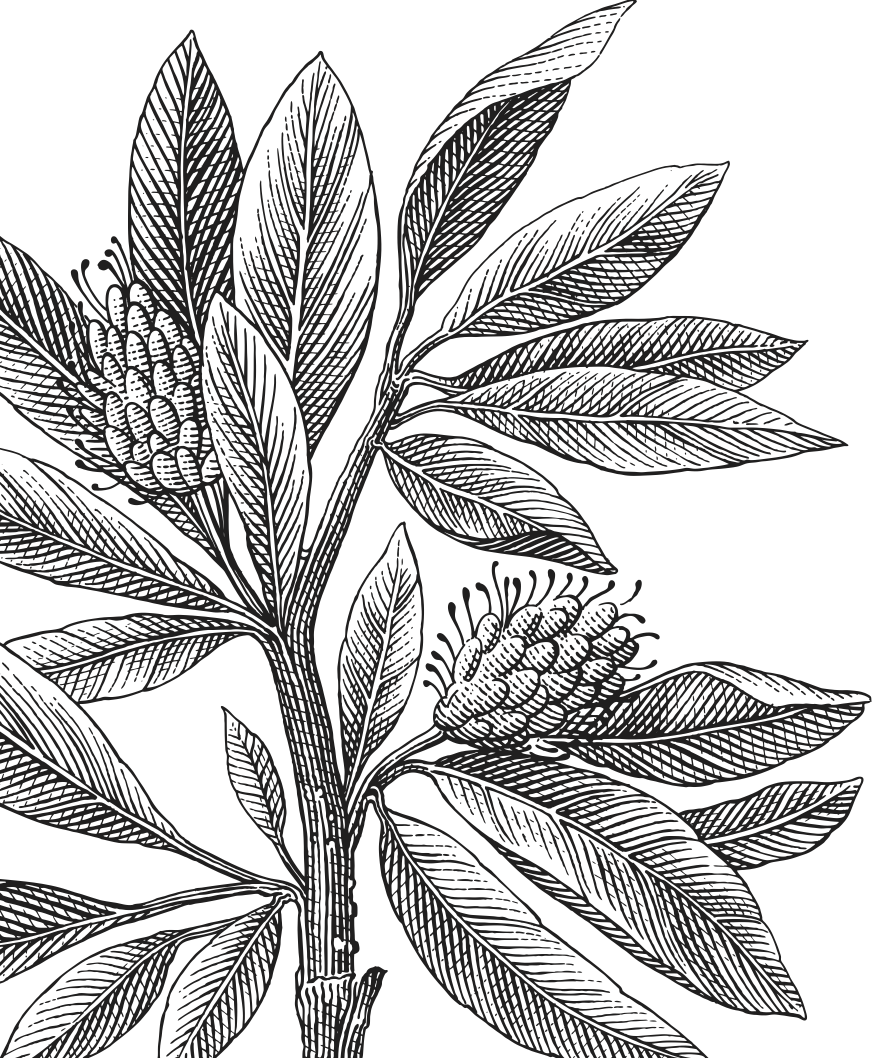
\includegraphics[keepaspectratio,scale=0.3]{img/lnu_etch.png} % Background image
    }
}
\newcommand\BackgroundPicLogo{
    \put(30,740){
    
\includegraphics[keepaspectratio,scale=0.10]{img/logo.png} % LNU logo
    }
}

\title{
\vspace{-8cm}
\begin{sidebar}
    \vspace{10cm}
    \normalfont \normalsize
    \huge Computer Technology I\\ % Main title
    \vspace{-1.3cm}
\end{sidebar}
\vspace{3cm}
\begin{flushleft}
    \huge Lab. 2 : How to use the PORTs, Digital input/output, Subroutine call % Subtitle
     \small \\ \emph{}
\end{flushleft}
\null
\vfill
\begin{textblock}{5}(10,13)
\begin{flushright}
\begin{minipage}{\textwidth}
\begin{flushleft} \large
\emph{Author:}\textsc{Anas Kwefati}\\  % Author
\emph{Supervisor:}  \textsc{Anders Haggren} \\  % Author
\emph{Semester:} Autumn 2019\\ % Semester
\emph{Area:} Computer Science \\ % Area
\emph{Course code:} 1DT301 % Course
\end{flushleft}
\end{minipage}
\end{flushright}
\end{textblock}
}

\date{} % Empty date command. Use \today inside for today's date.
\author{} % Normally one would use this to define authors. However in this case the title command takes care of everything, so we leave the field empty to get rid of warnings. 

\begin{document}

\pagenumbering{gobble} % Turn off page numbering
\newgeometry{left=5cm}
\AddToShipoutPicture*{\BackgroundPic} % Adds the background image to the title page
\AddToShipoutPicture*{\BackgroundPicLogo} % Adds the logo to the title page
\maketitle % Prints the title
\restoregeometry
\clearpage

\pagenumbering{roman} % Roman page numbering for abstract page


\selectlanguage{english}

\newpage

\pagenumbering{gobble} % Turn off page numbering
\tableofcontents 

\newpage
\pagenumbering{arabic} % Turn on page numbering


\section{Task 1}
For the first task the goal was to get a light blinking. This was done by setting the data direction register to output, and after that setting the LED port low.

\lstset{style=Asm}

\begin{lstlisting}
;>>>>>>>>>>>>>>>>>>>>>>>>>>>>>>>>>>>>>>>>>>>>>>>>>>>>>>>>>>>
; 1DT301, Computer Technology I
; Date: 2016-09-15
; Author:
;	Anas Kwefati
; Student name 2
;
; Lab number: 2
; Title: Subroutines
;
; Hardware: STK600, CPU ATmega2560
;
; Function: Program that switches between Ring counter and Johnson counter.
; 	No delay between the button is pressed and the change between Ring/Johnson.
; 	Each time I press the button, the program should change counter.

; Input ports: PORTA checks if we pressed the switch 0 (SW0; PA0).
;
; Output ports: PORTB turns on/off the light (LEDs)
;
; Subroutines: If applicable.
; Included files: m2560def.inc
;
; Other information:
;
; Changes in program: (Description and date)
;<<<<<<<<<<<<<<<<<<<<<<<<<<<<<<<<<<<<<<<<<<<<<<<<<<<<<<<<<<<

.include "m2560def.inc"

; Initialize SP, Stack Pointer
ldi r21, HIGH(RAMEND) ; R20 = high part of RAMEND address
out SPH,R21 ; SPH = high part of RAMEND address
ldi R21, low(RAMEND) ; R20 = low part of RAMEND address
out SPL,R21 ; SPL = low part of RAMEND address

;we initialize
ldi r16, 0xFF ;
out DDRB, r16 ; we set the DDRB as output

ldi r17, 0x00
out DDRA, r17 ; we set as output

ldi r16, 0xFF ; we load 0b1111 1111 to the register r16
out PORTA,r16 ; we set the PORTA to r16 SO it means that we put each light off

ldi r20, 0b11111110 ;check if we pressed SW0
ldi r19, 0b10111111 ;Turn on light at 0
ldi r22,0x00

loop:
	in r18, PINA ;we put the coming data received by the PIND(input) to r18
	cp r20,r18 ; check if r20==r18
	breq ring_counter
	brne johnson_counter


ring_counter:
	ldi r18, 0b11111110
	call ring_loop

ring_loop:
	out PORTB, r18 ;we put the value of r18 to PORTB which should turn on the light
	call Delay
	com r18
	LSL r18
	com r18

	;Check if everything is off if true then go to ring counter to make infinite loop
	ldi r24,0xFF
	cp r24, r18
	breq ring_counter

	in r19, PINA
	cp r20,r19
	breq johnson_counter

	rjmp ring_loop


rjmp loop ; we go back at the beginning of the infinite loop

johnson_counter :
	ldi r19, 0b11111110 ;Turn on light at 0
	ldi r22, 0x00

johnson_loop:
	out PORTB, r19
	LSL r19
	call Delay
	cp r19, r22
	breq johnson

;Check if PINA SW0 has been pressed if yes then it goes to ring counter
	in r18, PINA
	cp r20,r18
	breq ring_counter

	rjmp johnson_loop

rjmp loop ; we go back at the beginning of the infinite loop

johnson :
	out PORTB, r22
	ldi r22, 0b11111111
	call Delay
	ldi r19,0b10000000

	more_john :
		out PORTB, r19
		ASR r19
		call Delay
		cp r19, r22
		breq johnson_counter

;Check if PINA SW0 has been pressed if yes then it goes to ring counter
		in r18, PINA
		cp r20,r18
		breq ring_counter

	rjmp more_john



Delay :
; Generated by delay loop calculator
; at http://www.bretmulvey.com/avrdelay.html

	ldi  r21, 5
    ldi  r23, 20
    ldi  r24, 175
L1: dec  r24
    brne L1
    dec  r23
    brne L1
    dec  r21
    brne L1
	ret



	
\end{lstlisting}
\break

\begin{figure}
\begin{center}
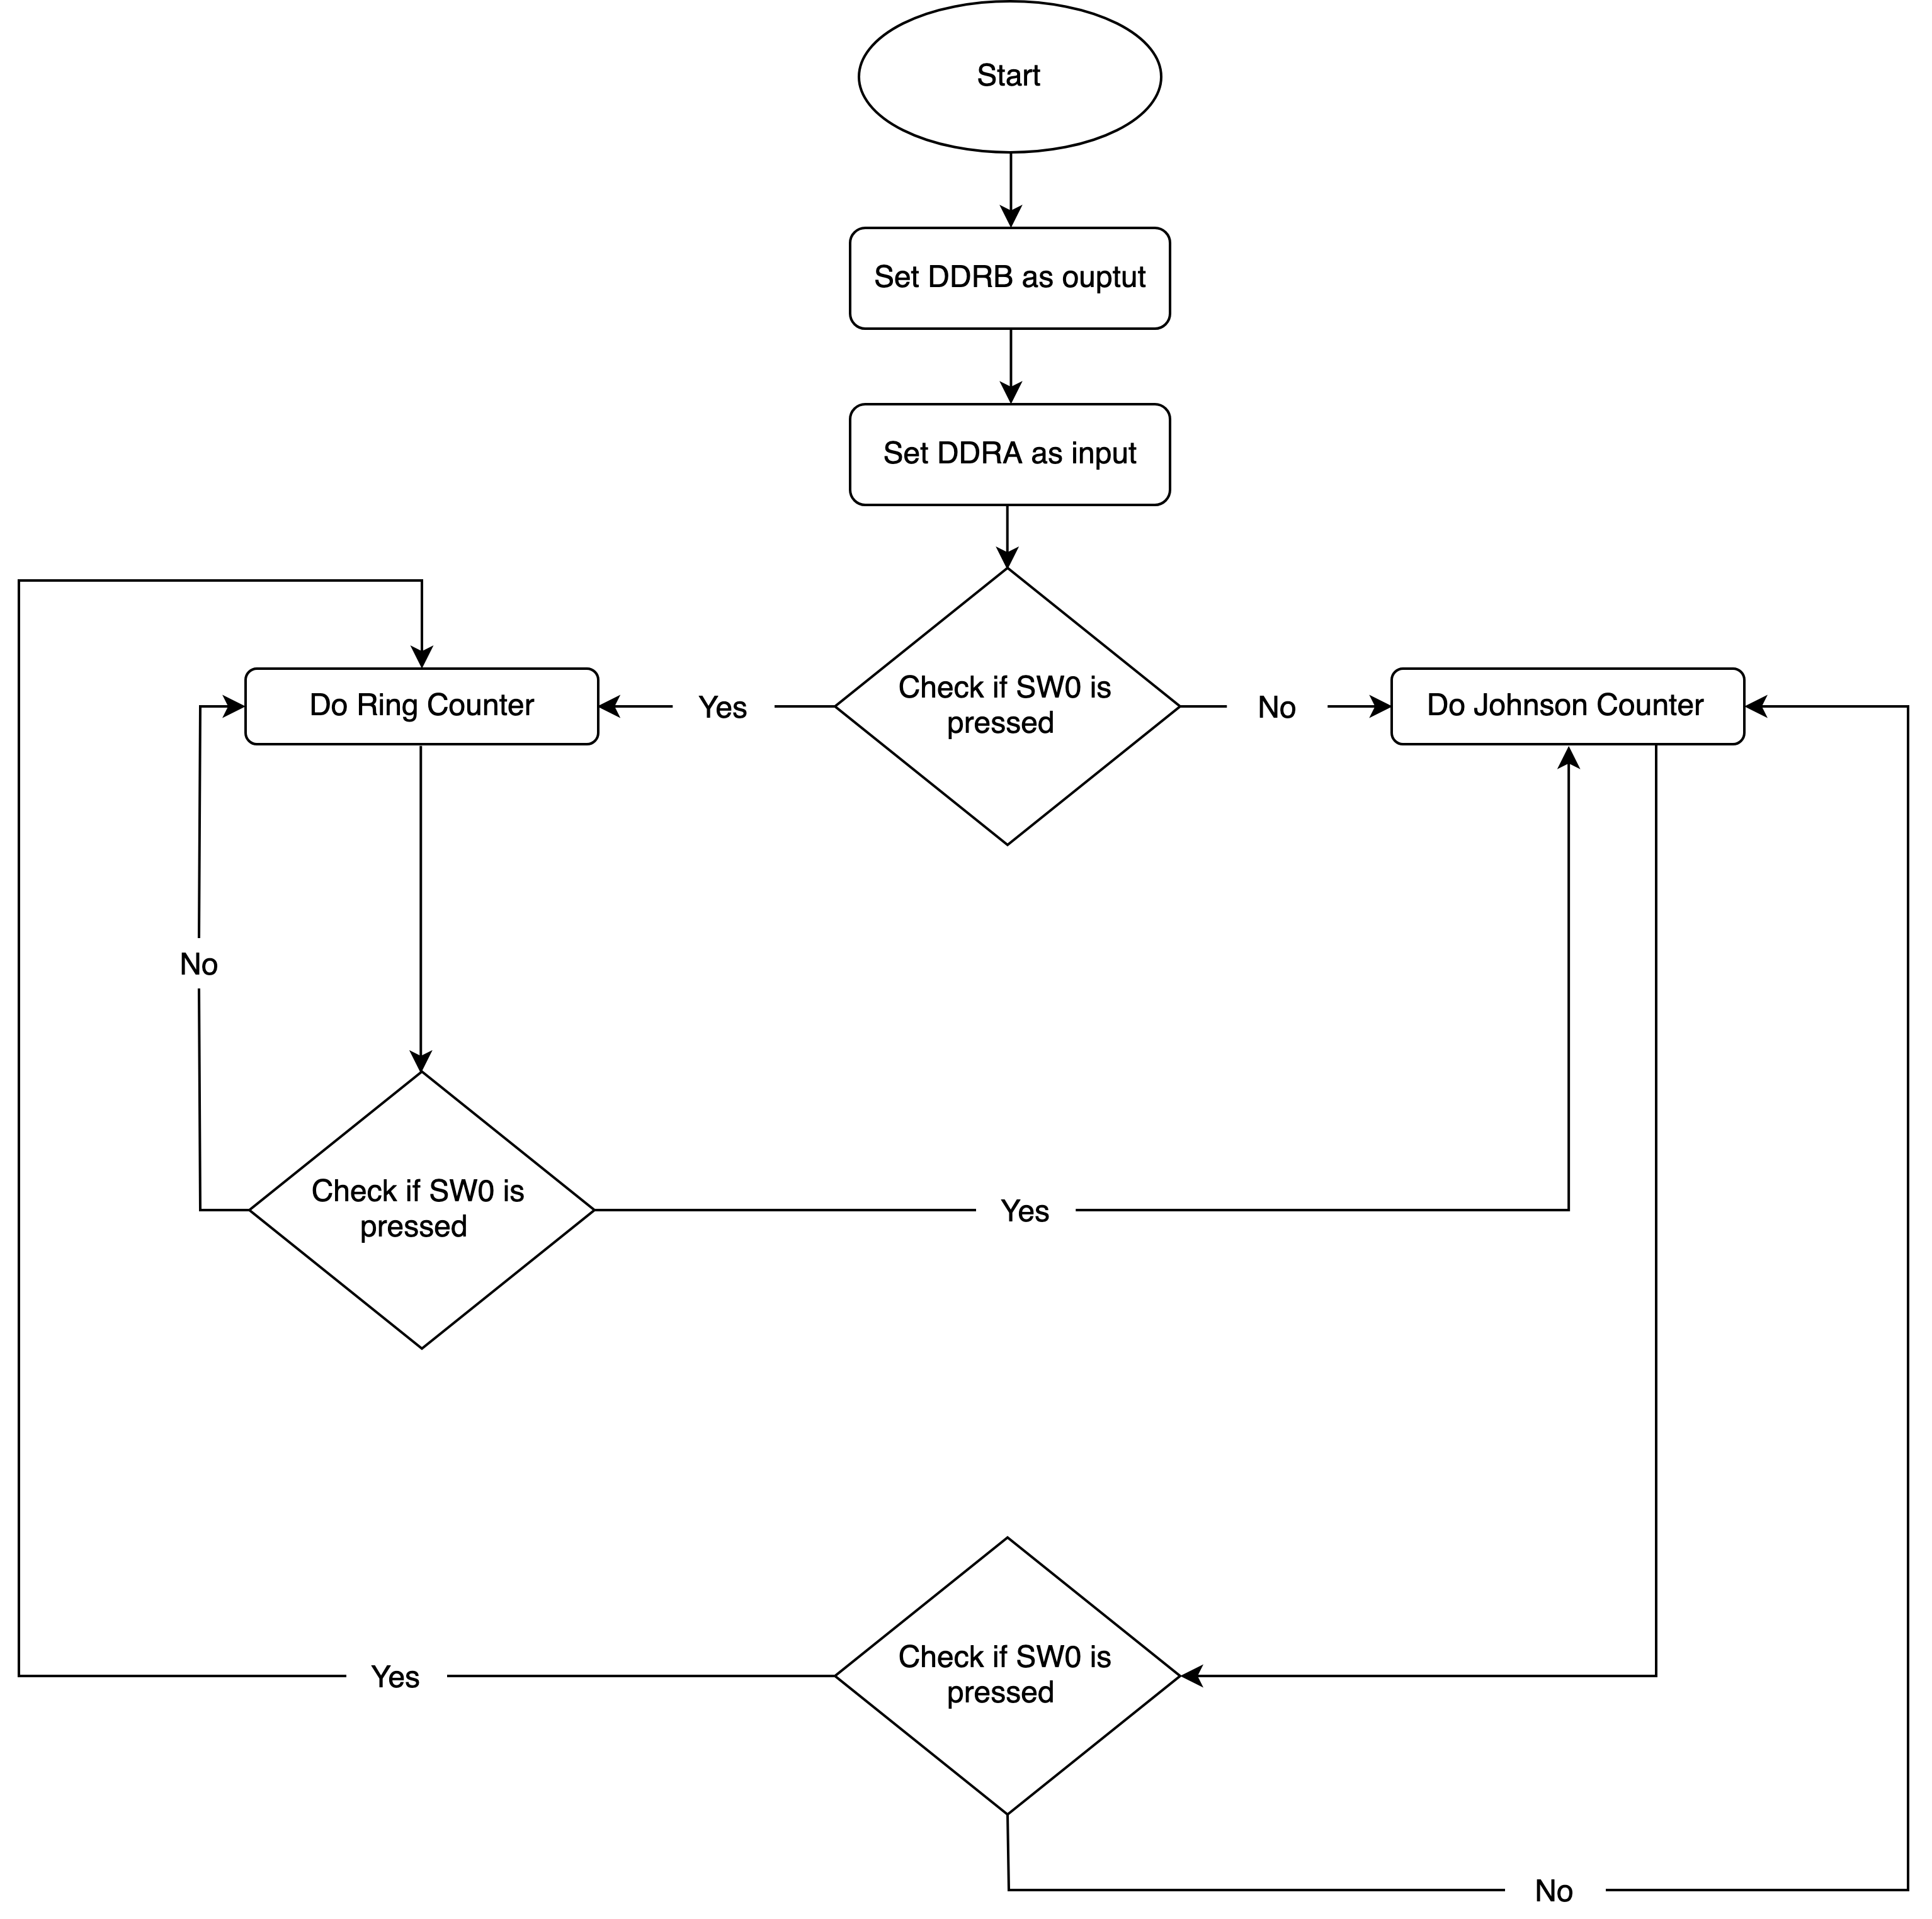
\includegraphics[width=\textwidth/3 ]{flowchart/task1_flowchart.png}
\end{center}
\caption{Task 1 flowchart}
\label{task1}
\end{figure}
\break



%TASK2
\section{Task 2}
For the second task the aim is to read switches and light to corresponding LED. This was done by using a data direction register 
\lstset{style=Asm}

\begin{lstlisting}
;>>>>>>>>>>>>>>>>>>>>>>>>>>>>>>>>>>>>>>>>>>>>>>>>>>>>>>>>>>>
; 1DT301, Computer Technology I
; Date: 2016-09-15
; Author:
;	Anas Kwefati
;
; Lab number: 2
; Title: Subroutines
;
; Hardware: STK600, CPU ATmega2560
;
; Function: Program that switches between Ring counter and Johnson counter.
; 	No delay between the button is pressed and the change between Ring/Johnson.
; 	Each time I press the button, the program should change counter.

; Input ports: PORTA checks if we pressed the switch 0 (SW0; PA0).
;
; Output ports: PORTB turns on/off the light (LEDs)
;
; Subroutines: If applicable.
; Included files: m2560def.inc
;
; Other information:
;
; Changes in program: (Description and date)
;<<<<<<<<<<<<<<<<<<<<<<<<<<<<<<<<<<<<<<<<<<<<<<<<<<<<<<<<<<<

.include "m2560def.inc"

; Initialize SP, Stack Pointer
ldi r21, HIGH(RAMEND) ; R20 = high part of RAMEND address
out SPH,R21 ; SPH = high part of RAMEND address
ldi R21, low(RAMEND) ; R20 = low part of RAMEND address
out SPL,R21 ; SPL = low part of RAMEND address

;we initialize
ldi r16, 0xFF ;
out DDRB, r16 ; we set the DDRB as output

ldi r17, 0x00
out DDRA, r17 ; we set DDRA as input


out PORTB, r16
ldi r18, 0b11111110
ldi r20, 1

ldi r16, 0b11111111

loop :
	in r19,PINA
	cp r19, r18
	breq listening_loop

rjmp loop


listening_loop :
	inc r20
	cpi r20, 7
	breq reset
	in r19, PINA
	cp r16,r19
	breq random
rjmp listening_loop

reset :
	ldi r20, 1
	rjmp loop

random :
	cpi r20, 1
	breq number_one
	cpi r20, 2
	breq number_two
	cpi r20, 3
	breq number_three
	cpi r20, 4
	breq number_four
	cpi r20, 5
	breq number_five
	cpi r20, 6
	breq number_six


number_one:
	ldi r22, 0b11111101
	out PORTB, r22
	rjmp loop

number_two:
	ldi r22, 0b10111101
	out PORTB, r22
rjmp loop
number_three:
	ldi r22, 0b10101011
	out PORTB, r22
rjmp loop
number_four:
	ldi r22, 0b00111001
	out PORTB, r22
rjmp loop
number_five:
	ldi r22, 0b00101001
	out PORTB, r22
rjmp loop
number_six:
	ldi r22, 0b00010001
	out PORTB, r22
rjmp loop


\end{lstlisting}
\break
\begin{figure}
\begin{center}
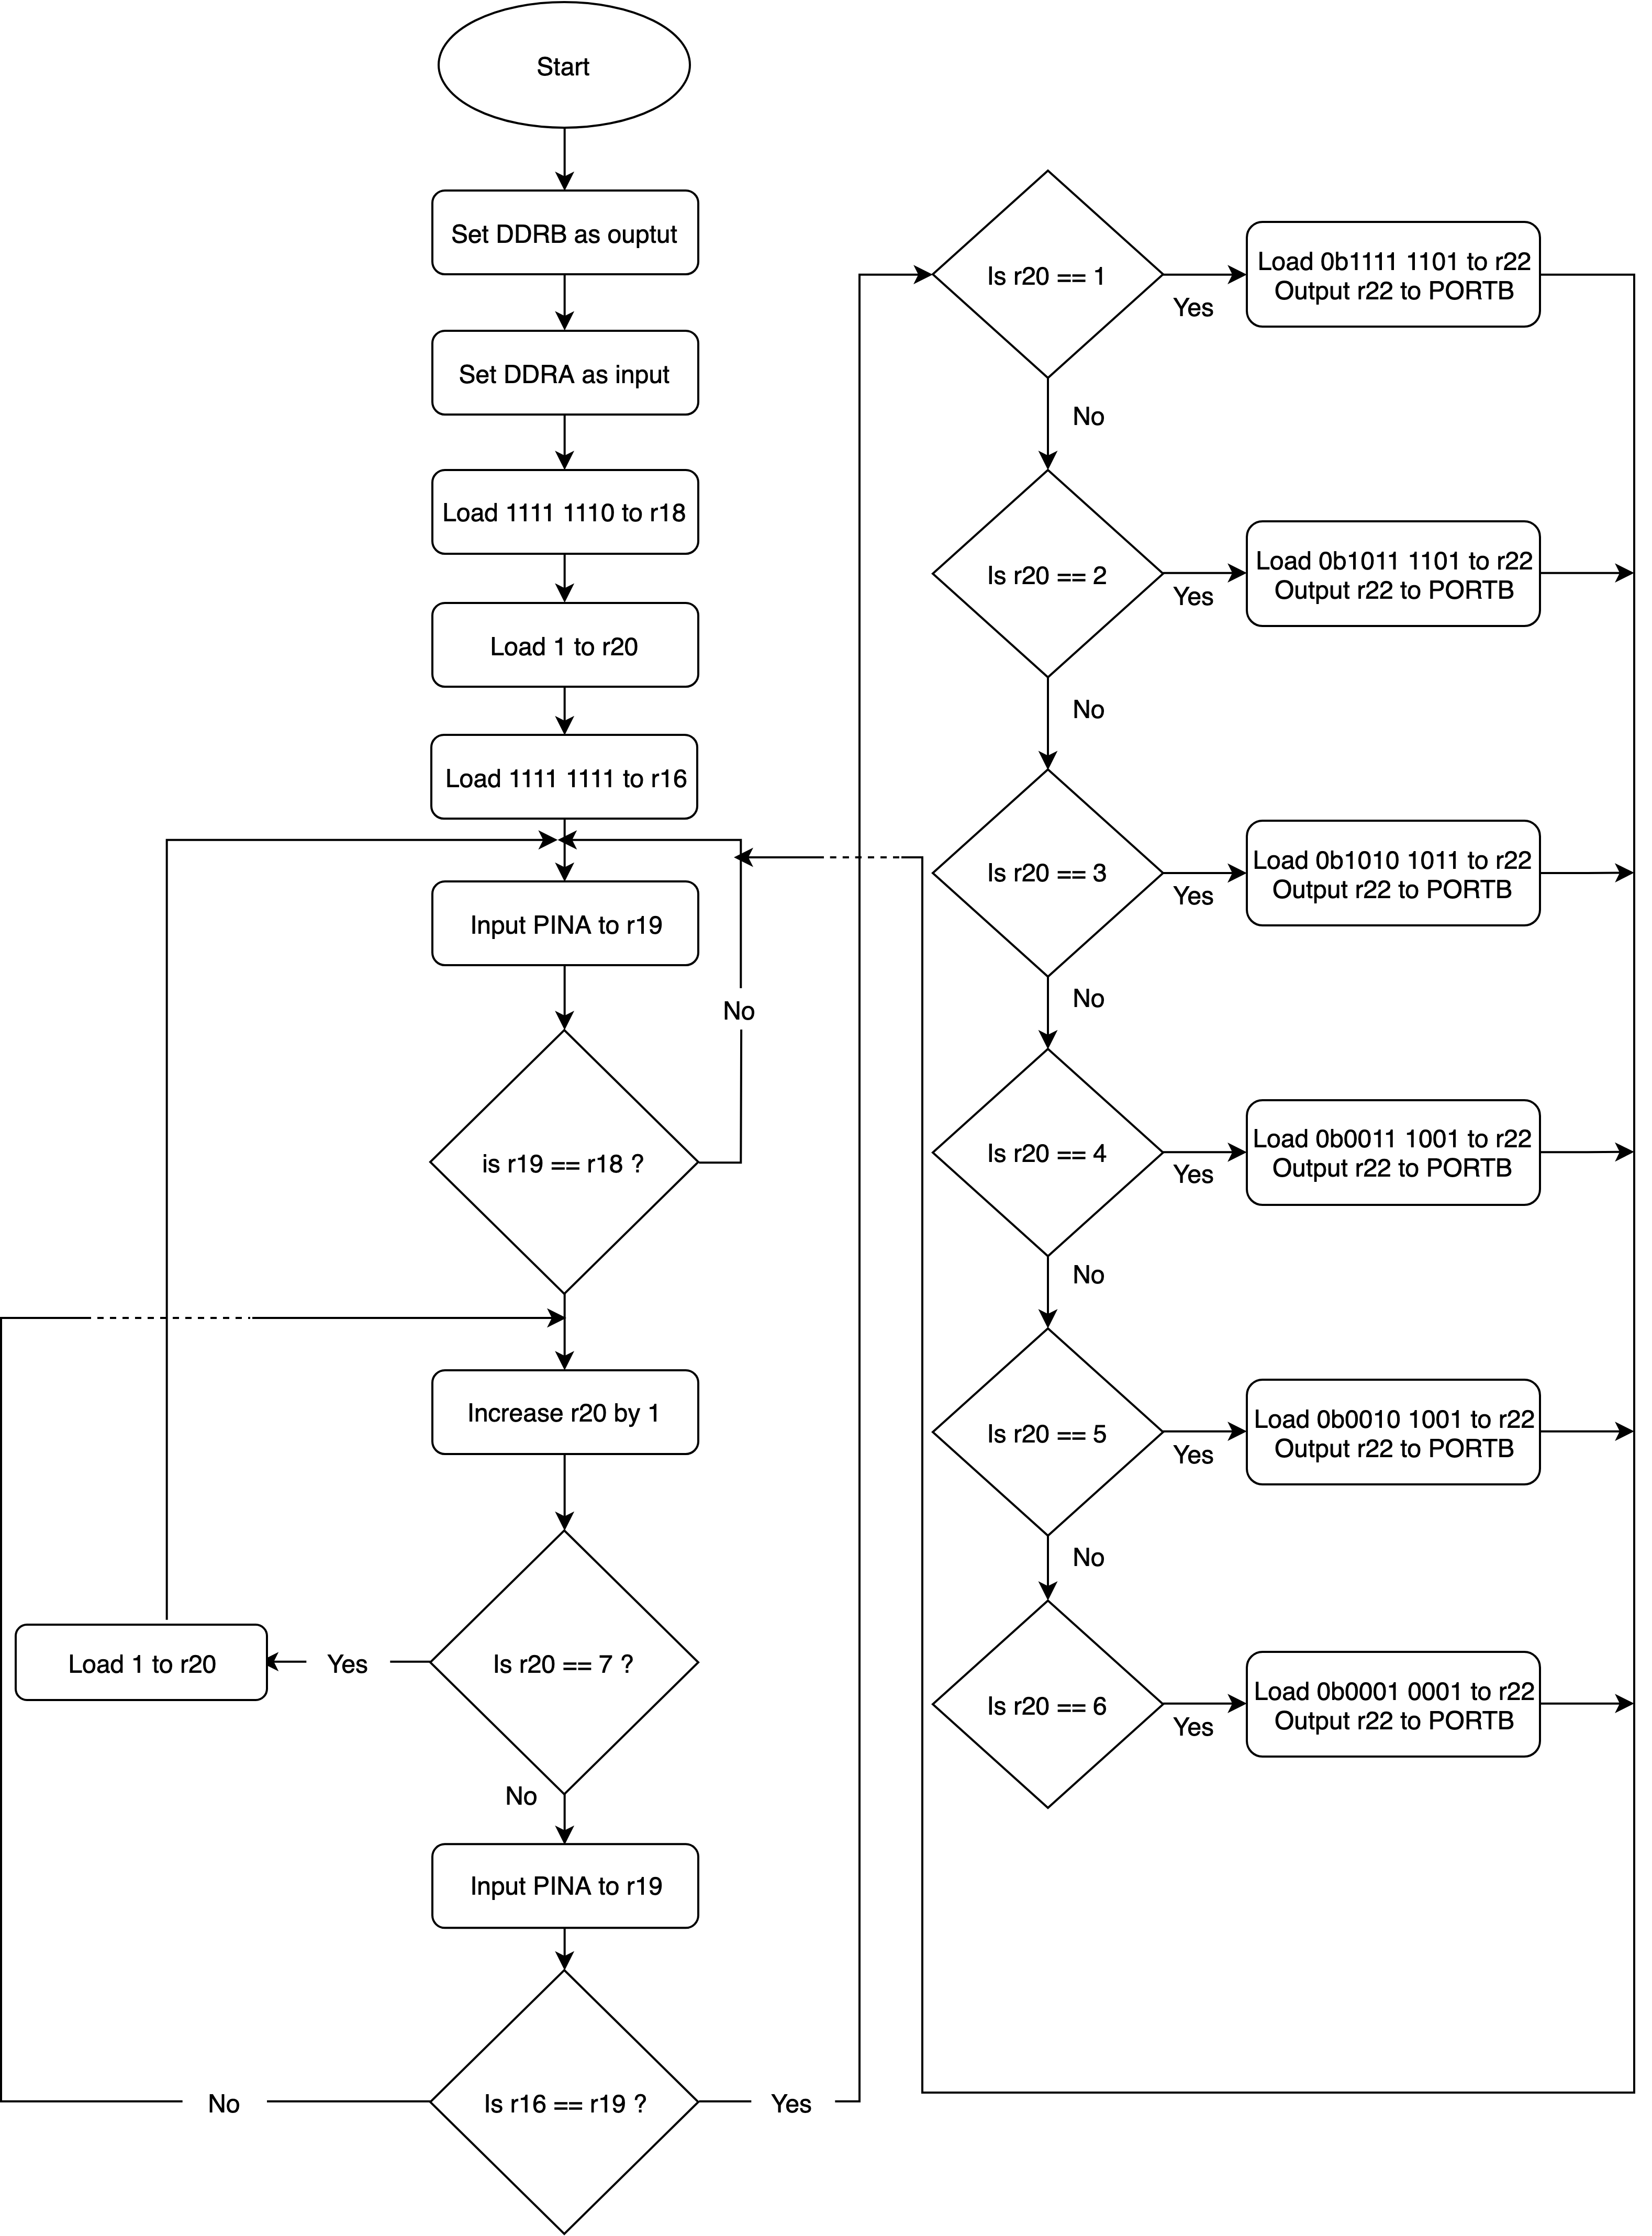
\includegraphics[width=\textwidth/3]{flowchart/task2_flowchart.png}
\end{center}
\caption{Task 2 flowchart}
\label{task2}
\end{figure}

\break

%TASK 3
\section{Task 3}
In task 3 the goal was to turn on led 0, only if switch 5 was pressed. by checking if the bit for switch 5 is high we are able to turn the led on at the right moment

\lstset{style=Asm}

\begin{lstlisting}
;>>>>>>>>>>>>>>>>>>>>>>>>>>>>>>>>>>>>>>>>>>>>>>>>>>>>>>>>>>>
; 1DT301, Computer Technology I
; Date: 2016-09-15
; Author:
;	Anas Kwefati
;
; Lab number: 2
; Title: Subroutines
;
; Hardware: STK600, CPU ATmega2560
;
; Function: Program that switches between Ring counter and Johnson counter.
; 	No delay between the button is pressed and the change between Ring/Johnson.
; 	Each time I press the button, the program should change counter.

; Input ports: PORTA checks if we pressed the switch 0 (SW0; PA0).
;
; Output ports: PORTB turns on/off the light (LEDs)
;
; Subroutines: If applicable.
; Included files: m2560def.inc
;
; Other information:
;
; Changes in program: (Description and date)
;<<<<<<<<<<<<<<<<<<<<<<<<<<<<<<<<<<<<<<<<<<<<<<<<<<<<<<<<<<<
.include "m2560def.inc"

; Initialize SP, Stack Pointer
ldi r21, HIGH(RAMEND) ; R20 = high part of RAMEND address
out SPH,R21 ; SPH = high part of RAMEND address
ldi R21, low(RAMEND) ; R20 = low part of RAMEND address
out SPL,R21 ; SPL = low part of RAMEND address

;we initialize
ldi r16, 0xFF ;
out DDRB, r16 ; we set the DDRB as output

ldi r17, 0x00
out DDRA, r17 ; we set DDRA as input

out PORTB, r16

ldi r18, 0b00000000 ; counter

ldi r19, 0b11111101 ; to check if button is pressed
ldi r23, 0xFF

loop :
	in r20, PINA
	cp r20,r19 ;compare r20 and r19
	breq counting ;if equal then go to counting
rjmp loop


counting :
	inc r18 ; we add +1

	mov r21, r18
	com r21

	out PORTB, r21

	counting_loop :

		in r20, PINA
		cp r20, r23

		breq whatever

		rjmp counting_loop

whatever :
	inc r18
	mov r21, r18
	com r21

	out PORTB, r21

	rjmp loop

\end{lstlisting}
\break
\begin{figure}
\begin{center}
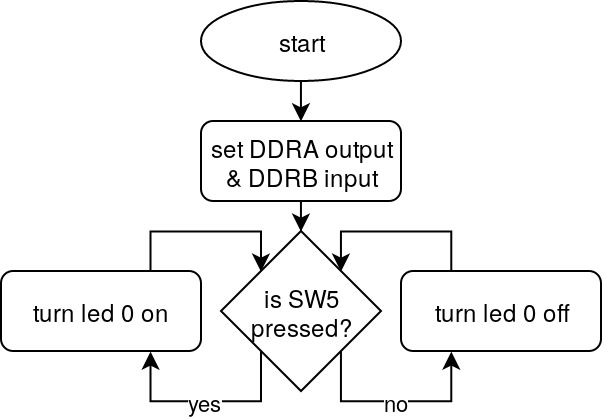
\includegraphics[width=\textwidth/2 ]{flowchart/task3_flowchart.jpg}
\end{center}
\caption{Task 3 flowchart}
\label{task3}
\end{figure}

\break

\section{Task 4}
For task 5 we needed to create a ring counter. This was done by creating a loop which constantly shifts the PORTB register one sideways with a delay.

\lstset{style=Asm}

\begin{lstlisting}
;>>>>>>>>>>>>>>>>>>>>>>>>>>>>>>>>>>>>>>>>>>>>>>>>>>>>>>>>>>>
; 1DT301, Computer Technology I
; Date: 2016-09-15
; Author:
; Student name 1
; Student name 2
;
; Lab number: 1
; Title: How to use the PORTs. Digital input/output. Subroutine call.
;
; Hardware: STK600, CPU ATmega2560
;
; Function: Describe the function of the program, so that you can understand it,
; even if you're viewing this in a year from now!
;
; Input ports: Describe the function of used ports, for example on-board switches
; connected to PORTA.
;
; Output ports: Describe the function of used ports, for example on-board LEDs
; connected to PORTB.
;
; Subroutines: If applicable.
; Included files: m2560def.inc
;
; Other information:
;
; Changes in program: (Description and date)
;<<<<<<<<<<<<<<<<<<<<<<<<<<<<<<<<<<<<<<<<<<<<<<<<<<<<<<<<<<<

.include "m2560def.inc"

; Initialize SP, Stack Pointer
ldi r21, HIGH(RAMEND) ; R20 = high part of RAMEND address
out SPH,R21 ; SPH = high part of RAMEND address
ldi R21, low(RAMEND) ; R20 = low part of RAMEND address
out SPL,R21 ; SPL = low part of RAMEND address

.equ nbrExecution = 2000 ; equ assigns a constant value to a label therefore this value cannot be changed later 
; we define the number of loop executions as constant 

;we initialize 
ldi r16, 0xFF ; 
out DDRB, r16 ; we set the DDRB as output

ring_counter:
	ldi r18, 0b11111110

ring_loop:
	out PORTB, r18 ;we put the value of r18 to PORTB which should turn on the light
	call Delay
	com r18
	LSL r18
	com r18

	;Check if everything is off if true then go to ring counter to make infinite loop
	ldi r21,0xFF
	cp r21, r18
	breq ring_counter
	rjmp ring_loop

Delay :
	
	; r25:r24 is a 16 bit register and so can have 65,536 different numbers, it can count 256 times longer than with an 8 bit register only. 

	;The lower byte of the 16-bit-adress is located in the lower register, the higher byte in the upper register. Both parts have their own names, e.g. the higher byte of Z is named ZH (=R31), the lower Byte is ZL (=R30). 
	;These names are defined in the standard header file for the chips. Dividing these 16-bit-pointer-names into two different bytes is done like follows:
	ldi r25, HIGH(nbrExecution) ; We set the Most Significant Bit at the address nbrExecution
	ldi r24, LOW(nbrExecution) ; We set the Least Significant Bit at the address nbrExecution

	wait_milliseconds :
		rcall sub_delay ;we call the sub_delay that contains 1ms that is going to be repeated 1000 times to do 1s
		sbiw r24, 1 ; By doing that we substract 1 from the register pair r25:r24
		;The instruction "SBIW R24,1" decreases the register pair word-wise. That means that whenever the LSB (Least Significant Bit r24) underflows, the MSB(Most Significant Bit r25) is also automatically reduced by 1.
		brne wait_milliseconds ; if not zero start loop again, if zero continue

	;rjmp wait_milliseconds ; as long as the pair value r25:r24 did not reach 0 it will stay in this wait_milliseconds loop
		


sub_delay : 
	; Generated by delay loop calculator
	; at http://www.bretmulvey.com/avrdelay.html
	;
	; Delay 2 000 cycles
	; 500us at 4.0 MHz

		ldi  r17, 3
		ldi  r19, 152
	L1: dec  r19
		brne L1
		dec  r17
		brne L1
		nop
		ret





\end{lstlisting}

Here is the flowchart for this task : 
\begin{center}
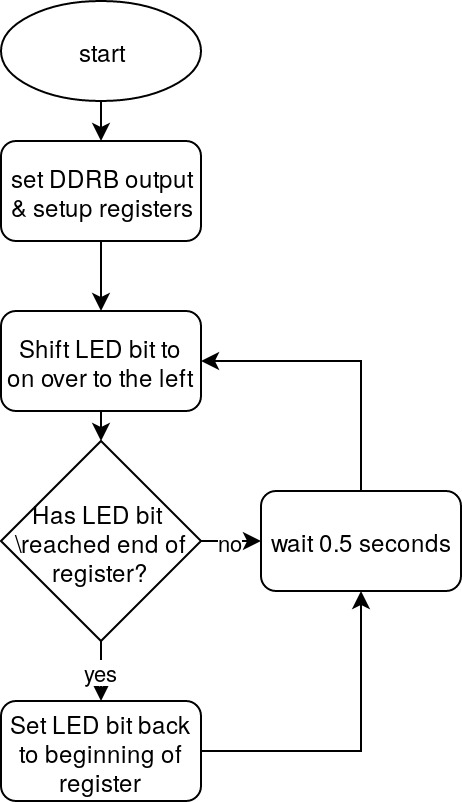
\includegraphics[width=\textwidth/2 ]{flowchart/task5_flowchart.jpg}

Task 5 flowchart
\label{task5}
\end{center}

\break 

% Prints your bibliography database xxx.bib
\bibliographystyle{IEEEtran}
\bibliography{ref.bib}

\end{document}
